\section{Analysis}
\label{sec:analysis}

Adversarial training often improves robustness at the cost of clean accuracy.
To mitigate this trade-off, we explore a self-distillation framework that does not begin with adversarial training, but instead first learns a clean self-teacher exclusively from natural images, thereby preserving a high-accuracy clean representation.
We then transfer the knowledge of this clean self-teacher to the student while adversarially training the student for robustness.
A central question is therefore how the knowledge encoded by the clean self-teacher should be transferred under adversarial perturbations.
We first revisit predictive distillation, where the teacher's softened output distribution serves as the supervision target, as commonly adopted in adversarial distillation.
In contrast, we study direct distillation of the clean self-teacher's feature representation and analyze how a fixed clean feature anchor jointly constrains clean-teacher fidelity and local feature variation.


\subsection{Preliminaries}

Let \(x\in\mathcal X=[0,1]^D\) denote a clean input, and define its \(\ell_\infty\)-bounded perturbation set as
\begin{equation}
B(x,\epsilon)
=
\{x'\in\mathcal X:\lVert x'-x\rVert_\infty\le\epsilon\},
\end{equation}
where \(x'\) denotes a perturbed input within the \(\epsilon\)-neighborhood of \(x\).
During adversarial training, \(x'\) is chosen to maximize the corresponding student loss over \(B(x,\epsilon)\).

We decompose a network as \(f=h\circ\Phi\), where
\(\Phi:\mathcal X\to\mathbb R^d\) is a continuous feature map and
\(h:\mathbb R^d\to\mathbb R^C\), \(h(z)=Wz+b\), is the classifier for \(C\) classes.
We use subscripts \(t\) and \(s\) for the frozen clean self-teacher and the student, respectively.
Both networks share the same architecture, with fixed network statistics for the analysis; feature distances are Euclidean unless stated otherwise.


\subsection{From Soft Predictive Targets to a Fixed Clean Target}
\label{sec:fragile}

Soft-label robust distillation transfers the clean teacher's knowledge through its predictive distribution, typically controlled by a temperature parameter \(\tau\) \citep{ard,rslad,adr,bmtard}.
Given a clean input \(x\) and a perturbed input \(x'\in B(x,\epsilon)\), we define
\begin{equation}
q_t^\tau(x)
=
\operatorname{softmax}(f_t(x)/\tau),
\qquad
p_s^\tau(x')
=
\operatorname{softmax}(f_s(x')/\tau),
\label{eqn:soft_targets}
\end{equation}
where the teacher is evaluated on the clean input \(x\), whereas the student is evaluated on its perturbed counterpart \(x'\).

Conventional knowledge distillation applies the same temperature to both distributions and minimizes the scaled divergence
\begin{equation}
\mathcal L_{\mathrm{KD}}^\tau(x,x')
=
\tau^2
D_{\mathrm{KL}}
\bigl(q_t^\tau(x)\|p_s^\tau(x')\bigr).
\label{eqn:kd_variants}
\end{equation}

Increasing \(\tau\) makes both predictive distributions progressively softer.
In particular, the clean teacher target \(q_t^\tau(x)\) approaches the uniform distribution as \(\tau\to\infty\), and its entropy approaches the maximum value \(\log C\), as illustrated in \Cref{fig:targetcomparison}a.
This does not imply that the shared-temperature KD objective loses all information about the teacher.
Although both distributions become nearly uniform, their deviations from uniformity still encode the relative structure of the underlying logits.

More precisely, for fixed logits and
\[
\bar f
=
f-C^{-1}\mathbf 1\mathbf 1^\top f,
\]
the conventional \(\tau^2\) scaling preserves this residual information in the high-temperature limit:
\begin{equation}
\lim_{\tau\to\infty}
\tau^2
D_{\mathrm{KL}}
\bigl(q_t^\tau(x)\|p_s^\tau(x')\bigr)
=
\frac{1}{2C}
\lVert
\bar f_t(x)-\bar f_s(x')
\rVert_2^2.
\label{eqn:kd_limit}
\end{equation}

Thus, while the softened probabilities themselves approach uniformity, their scaled discrepancy converges to the squared distance between the centered teacher and student logits.
The centering reflects the shift invariance of softmax: adding the same constant to every logit does not change the predictive distribution.
Consequently, high-temperature predictive distillation approaches direct regression of the perturbed student's logits onto the clean self-teacher's logits, up to a common shift.

This connection motivates a more direct view of knowledge transfer.
Rather than passing the clean teacher's knowledge through a softened predictive distribution, we can directly regress the student onto a fixed clean target.
The high-temperature limit naturally gives a logit-level realization of this principle.
CFA instead applies it at the representation level by anchoring the student's perturbed feature to the clean self-teacher feature:
\begin{equation}
\mathcal L_{\mathrm{anchor}}(x)
=
\max_{x'\in B(x,\epsilon)}
\lVert
\Phi_s(x')-\Phi_t(x)
\rVert_2^2.
\label{eqn:anchor_percell}
\end{equation}

Here, \(\Phi_t(x)\) is computed from the clean input and serves as the fixed target, whereas the student is optimized against the worst-case perturbed input within \(B(x,\epsilon)\).
Logit regression constrains the representation through the classifier output, while feature regression directly constrains the representation supplied to the inherited classifier.
We empirically compare these two realizations below.


\begin{figure}[!htbp]
  \centering
  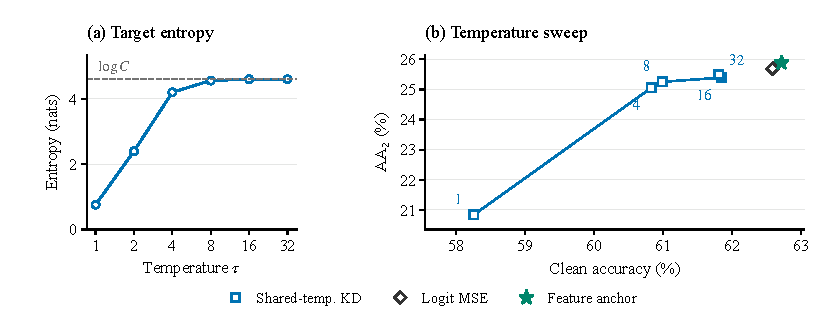
\includegraphics[width=\linewidth]{figure/analysis_targets.pdf}
  \caption{
  Target comparison on CIFAR-100 (ResNet-18).
  (a) Entropy of the clean teacher target \(q_t^\tau(x)\), which approaches the uniform entropy \(\log C\) as the shared temperature \(\tau\) increases.
  (b) Clean accuracy and AA under shared-temperature KD for different values of \(\tau\), together with direct logit and feature regression.
  Numbers denote \(\tau\).
  The full temperature sweep is reported in \Cref{tab:targetcomparison_values}.
  }
  \label{fig:targetcomparison}
\end{figure}


We next compare these forms of supervision to examine how the transition from predictive distillation to direct clean-target regression affects the clean--robust trade-off.
All variants are trained for 50 epochs under an \(\ell_\infty\) perturbation budget of \(\epsilon=8/255\).

As shown in \Cref{fig:targetcomparison}b, increasing the shared temperature moves the KD solution toward the operating point obtained by direct logit regression, consistent with the high-temperature limit in \Cref{eqn:kd_limit}.
This occurs even as the teacher target becomes nearly uniform at large \(\tau\) (\Cref{fig:targetcomparison}a), because the scaled discrepancy retains the relative structure of the underlying logits.

Direct feature regression yields \(0.13\) and \(0.19\) percentage-point improvements in clean accuracy and AA, respectively, over logit regression.
Under the final training recipe, the corresponding differences remain small at \(0.26/0.13\) points (\Cref{tab:finalallocation}).
Thus, direct regression onto a fixed clean target provides a temperature-free alternative to predictive distillation, while the small gap between logit and feature regression does not by itself establish an inherent empirical advantage of feature coordinates.

We also note that KD updates the classifier, whereas the regression variants keep it fixed.
The comparison therefore evaluates complete training designs rather than isolating the target representation alone.

\label{sec:sole_target}

The comparison shifts our focus from how a predictive distribution should be softened to what is controlled by anchoring the student to a fixed clean target.
We next characterize this fixed-anchor property for the feature-space realization used by CFA.


\subsection{What the Anchor Controls}
\label{sec:decomp}

CFA is designed to preserve the representation of the clean self-teacher while the student is trained against adversarial perturbations.
We therefore ask what controlling the fixed-anchor objective implies about the student's representation.
In particular, a desirable student should remain faithful to the clean teacher at the original input while exhibiting limited feature variation within the perturbation set.

To formalize these properties, let \(x\in\mathcal X\) and \(B=B(x,\epsilon)\), and define
\begin{equation}
L
=
\max_{x'\in B}
\lVert\Phi_s(x')-\Phi_t(x)\rVert_2,
\qquad
F
=
\lVert\Phi_s(x)-\Phi_t(x)\rVert_2,
\qquad
O
=
\max_{x',x''\in B}
\lVert\Phi_s(x')-\Phi_s(x'')\rVert_2.
\label{eqn:LFO}
\end{equation}

Here, \(L\) is the worst-case discrepancy from the fixed clean teacher anchor and corresponds to the quantity directly controlled by the CFA objective.
\(F\) measures the clean feature discrepancy between the student and its self-teacher, capturing the fidelity of the transferred clean representation.
\(O\) measures the diameter of the student's feature set over the perturbation region and thus its local feature variation.

These quantities satisfy the following relation.

\begin{proposition}[Fixed-anchor decomposition]
\label{prop:decomp}
For every \(x\in\mathcal X\) and \(\epsilon\ge0\),
\begin{equation}
L
\le
F+O
\le
3L.
\label{eqn:decomp}
\end{equation}
\end{proposition}

\begin{proof}
For any \(x'\in B\), the triangle inequality gives
\[
\lVert\Phi_s(x')-\Phi_t(x)\rVert_2
\le
\lVert\Phi_s(x')-\Phi_s(x)\rVert_2
+
\lVert\Phi_s(x)-\Phi_t(x)\rVert_2
\le
O+F.
\]
Maximizing over \(x'\in B\) yields \(L\le F+O\).

Conversely, since \(x\in B\),
\[
F
=
\lVert\Phi_s(x)-\Phi_t(x)\rVert_2
\le L.
\]
Moreover, for any \(x',x''\in B\),
\[
\begin{aligned}
\lVert\Phi_s(x')-\Phi_s(x'')\rVert_2
&\le
\lVert\Phi_s(x')-\Phi_t(x)\rVert_2
+
\lVert\Phi_s(x'')-\Phi_t(x)\rVert_2 \\
&\le
2L.
\end{aligned}
\]
Hence \(O\le2L\), and therefore \(F+O\le3L\).
\end{proof}

The proposition gives a direct interpretation of the CFA objective.
If \(L\le\delta\), then
\[
F\le\delta,
\qquad
O\le2\delta.
\]
Thus, keeping the worst-case student feature close to the clean teacher anchor simultaneously keeps the student's clean representation close to the teacher and limits feature variation throughout the perturbation region.
Importantly, this conclusion does not require the clean teacher itself to be robust or locally stable; only its representation at the clean input \(\Phi_t(x)\) serves as the anchor.

Because CFA inherits the teacher's linear classifier, the same discrepancy also bounds the deviation at the classifier output.
For \(h_t(z)=W_tz+b_t\),
\begin{equation}
\lVert
h_t(\Phi_s(x'))
-
h_t(\Phi_t(x))
\rVert_2
\le
\lVert W_t\rVert_{2\rightarrow2}
\lVert
\Phi_s(x')-\Phi_t(x)
\rVert_2
\le
\lVert W_t\rVert_{2\rightarrow2}L.
\end{equation}
A small anchor discrepancy therefore limits how far the student's logits can deviate from the clean teacher logits under the inherited classifier.
This bound alone does not guarantee identical predictions, which additionally depend on the teacher's clean classification margin.

The fixed-anchor argument is not specific to feature coordinates and analogously applies to norm-based regression onto a fixed logit target.
It therefore characterizes the joint control induced by a fixed target rather than establishing an inherent advantage of feature matching.
In practice, finite-step PGD only approximates the inner maximization and thus does not certify the true value of \(L\).

\FloatBarrier


\subsection{How Does Teacher Performance Affect Transfer?}
\label{sec:teacher_transfer}
\label{sec:geometry}

The preceding analysis shows that anchoring the student to a fixed clean target can preserve its agreement with the self-teacher while limiting local feature variation.
This raises a natural question about the teacher itself: does a better-performing clean self-teacher necessarily provide a better target for robust transfer?

A straightforward expectation is that a teacher with higher clean accuracy should provide stronger clean supervision and consequently yield a better student.
We first examine this hypothesis using different checkpoints along the training trajectory of the same clean self-teacher.
Because each checkpoint determines the student's initialization, feature target, and inherited classifier, this experiment measures the combined effect of the teacher state transferred to the student.


\begin{figure}[!htbp]
  \centering
  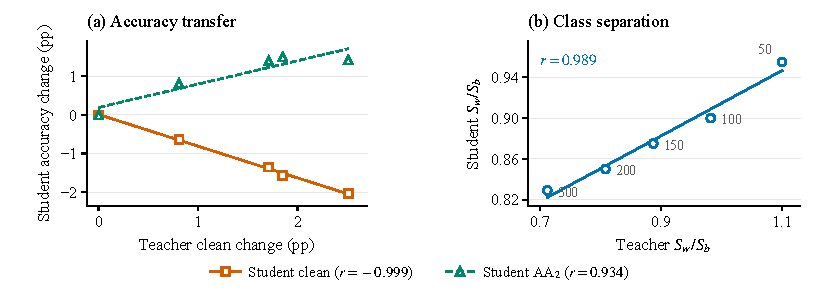
\includegraphics[width=\linewidth]{figure/teacher_checkpoint_trends.pdf}
  \caption{
  Transfer from clean self-teachers at different stages of training on CIFAR-100 (ResNet-18).
  (a) Changes in teacher clean accuracy and resulting student clean accuracy and AA relative to the 50-epoch teacher.
  (b) Within-to-between scatter ratios \(S_w/S_b\) of teacher and student features; lower values indicate stronger class separation, and labels denote teacher epochs.
  Lines are least-squares fits.
  Exact values are reported in \Cref{tab:teacherladder_values}.
  }
  \label{fig:teacherladder}
\end{figure}


As the clean self-teacher is trained from 50 to 300 epochs, its clean accuracy increases by \(2.51\) percentage points.
This improvement, however, does not translate into a simultaneous improvement in the student's clean and robust performance.
Student clean accuracy decreases by \(2.04\) points, while AA increases from \(24.38\%\) to \(25.80\%\) (\Cref{fig:teacherladder}a).
Thus, increasing teacher clean accuracy shifts the student's clean--robust operating point rather than uniformly improving it.
The trend is also not strictly monotonic: the student transferred from the 200-epoch teacher achieves slightly higher AA than that transferred from the 300-epoch teacher.

To examine whether this behavior is specific to a single teacher trajectory, we repeat the experiment with an independently trained clean self-teacher.
The same overall pattern emerges.
From 40 to 300 teacher epochs, teacher clean accuracy increases from \(75.57\%\) to \(78.27\%\), whereas student clean accuracy decreases from \(64.36\%\) to \(62.34\%\) and AA increases from \(23.86\%\) to \(25.94\%\) (\Cref{tab:teachertrajectory}).
Across both trajectories, higher teacher clean accuracy therefore accompanies a shift in the student's clean--robust trade-off rather than a uniform improvement in student performance.


\begin{table}[!htbp]
  \centering
  \small
  \setlength{\tabcolsep}{6pt}
  \caption{
  Transfer from an independently trained clean self-teacher trajectory on CIFAR-100 (ResNet-18; 50-epoch students).
  Full results are reported in \Cref{tab:teacherladder_seed1}.
  }
  \label{tab:teachertrajectory}
  \begin{tabular}{rrrrr}
    \toprule
    Teacher epoch & Teacher clean & Student clean & Student AA & Student NRR \\
    \midrule
    40  & 75.57 & 64.36 & 23.86 & 34.81 \\
    100 & 77.27 & 63.68 & 25.61 & 36.53 \\
    200 & 77.90 & 63.02 & 26.16 & 36.97 \\
    300 & 78.27 & 62.34 & 25.94 & 36.64 \\
    \bottomrule
  \end{tabular}
\end{table}


Teacher clean accuracy alone does not reveal what changes in the transferred representation as training progresses.
To examine the representation associated with this shift, we measure the within-to-between scatter ratio \(S_w/S_b\) on unit-normalized clean features.
As shown in \Cref{fig:teacherladder}b, the teacher and student ratios decrease together as teacher training progresses, indicating increasingly separated class structure in both representations.
This association suggests that changes in the teacher representation are reflected in the resulting student, but does not identify which representational property causes the observed clean--robust shift.

The checkpoint comparison couples teacher accuracy with training stage and other changes in the learned representation.
We therefore further ask whether clean accuracy alone is sufficient to characterize a teacher for transfer.
To separate teacher accuracy from training stage, we compare clean self-teachers trained with label smoothing and mixup that achieve nearly identical clean accuracy.


\begin{table}[!htbp]
  \centering
  \small
  \setlength{\tabcolsep}{4.5pt}
  \caption{
  Transfer from accuracy-matched clean self-teachers on CIFAR-100 (ResNet-18; 50-epoch students).
  Feature sensitivity is measured on held-out data.
  }
  \label{tab:matchedteacher}
  \begin{tabular}{lrrcrr}
    \toprule
    & \multicolumn{2}{c}{Teacher} && \multicolumn{2}{c}{Student} \\
    \cmidrule(lr){2-3}\cmidrule(lr){5-6}
    Natural training & Clean & Sensitivity && Clean & AA \\
    \midrule
    Label smoothing \(0.1\) & 78.76 & 3.16 && 59.62 & 25.72 \\
    Mixup                 & 78.62 & 4.82 && 63.80 & 25.70 \\
    \bottomrule
  \end{tabular}
\end{table}


Despite differing by only \(0.14\) percentage points in teacher clean accuracy, the two teachers produce students whose clean accuracies differ by \(4.18\) points, while their AA differs by only \(0.02\) points (\Cref{tab:matchedteacher}).
Teacher clean accuracy is therefore insufficient to characterize how the clean representation will transfer to the adversarially trained student.
The teachers also differ in feature sensitivity in the same order as student clean accuracy, suggesting that properties of the transferred representation beyond teacher accuracy may be relevant.
With only one accuracy-matched pair, however, this observation is insufficient to establish feature sensitivity as a general predictor of transfer.

Taken together, these results show that the role of the clean self-teacher cannot be summarized by its clean accuracy alone.
As the teacher representation evolves, the resulting student can move to a different point on the clean--robust trade-off even as teacher clean accuracy improves, and teachers with nearly matched clean accuracy can transfer differently.
We use the 200-epoch clean self-teacher for the subsequent experiments and next consider a source of variation that remains after the teacher is fixed: the same perturbation radius need not induce the same anchor discrepancy across individual examples.